\section{Overview}
\label{sec:overview}

\begin{figure} 
\begin{verbatim}
var Color: int; // WHITE=1, GRAY=2, BLACK=3
procedure WB(linear tid:Tid)
atomic [if (Color == WHITE) Color := GRAY];
{
  var cNoLock:int;
  cNoLock := GetColorNoLock(tid);
  yield Color >= cNoLock;
  if (cNoLock == WHITE) 
    call WBSlow(tid);
}
procedure WBSlow(linear tid:Tid)
atomic [if (Color == WHITE) Color := GRAY];
{
  var cLock:int;
  call AcquireLock(tid);
  cLock := GetColorLocked(tid);
  if (cLock == WHITE) 
    call SetColorLocked(tid, GRAY);
  call ReleaseLock(tid);
}
procedure GetColorNoLock(linear tid:Tid) 
  returns (cl:int) atomic [...];
procedure AcquireLock(linear tid:Tid) 
  right [...];
procedure ReleaseLock(linear tid:Tid) 
  left [...];
procedure GetColorLocked(linear tid:Tid) 
  returns (cl:int) both [...];
procedure SetColorLocked(linear tid:Tid, 
  cl: int) atomic [...];
\end{verbatim}
\caption{Write barrier}
\label{fig:reft}
\end{figure}


We present an overview of our approach to refinement on the program in Figure~\ref{fig:reft},
a simplified version of the write barrier in a concurrent garbage collector (GC).
In a concurrent GC, a color (either \exC{WHITE}, \exC{GRAY}, or \exC{BLACK})
is associated with each object on the heap.  
Before writing to an address \exC{addr}, a mutator executes a write
barrier. It checks 
\exC{addr} has color \exC{WHITE}
and sets it to \exC{GRAY}, indicating that the object at \exC{addr}
and objects reachable from it should not be garbage collected. 

\begin{figure}
\begin{center}
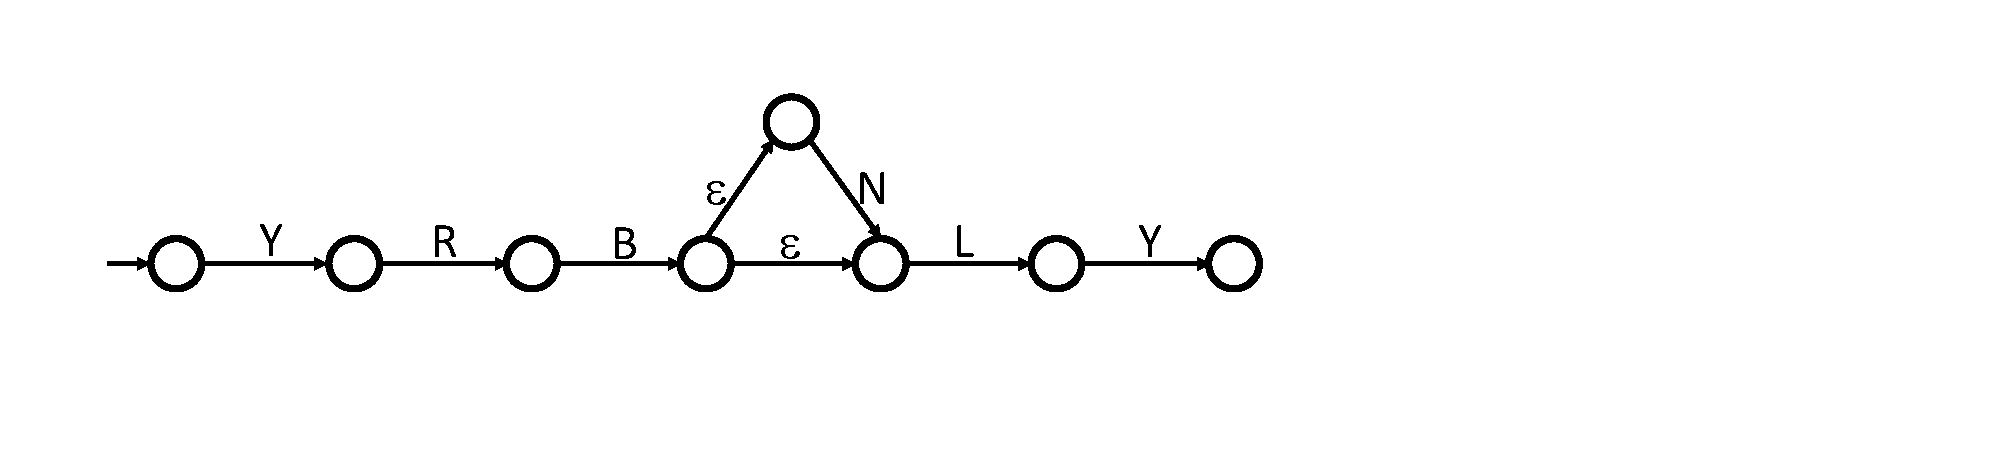
\includegraphics[scale=0.35]{WBSlow.pdf}
\end{center}
\caption{Abstraction of \exC{WBSlow}}
\label{fig:midwb}
\end{figure}
 
Procedure \exC{WB} implements the write barrier.
To simplify exposition, 
we consider a single object whose color is stored in the shared variable \exC{Color}.
\exC{WB} first reads \exC{Color} without holding a lock, to avoid,
when possible, the
cost of acquiring and releasing a lock for each address encountered by
a mutator. 
If \exC{Color} is {\tt WHITE}, it calls the more expensive procedure \exC{WBSlow} 
to re-examines and possibly update \exC{Color} while holding the lock.
\civl simplifies reasoning about \exC{WB} and \exC{WBSlow} by allowing us to 
compactly express their specification as the following atomic action:\\

\begin{tt}
[if (Color == WHITE)  Color := GRAY]
\end{tt}

This specification indicates that regardless of the different implementations of 
\exC{WB} and \exC{WBSlow} and regardless of how the environment interferes
with their execution, to their respective callers it appears as if they atomically execute the above code.

\begin{figure}
\begin{center}
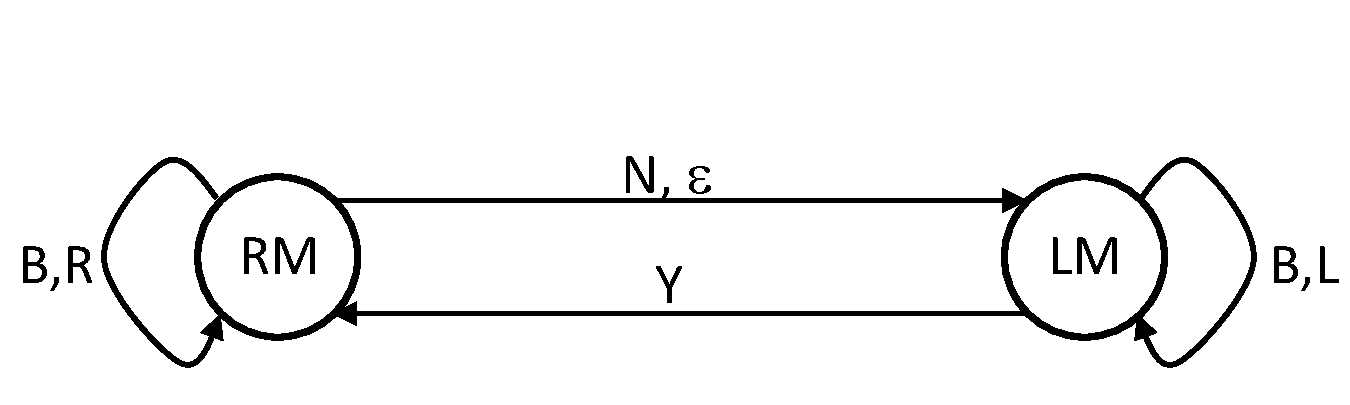
\includegraphics[scale=0.35]{YieldTypeCheckingAutomaton.pdf}
\end{center}
\caption{Yield sufficiency automaton ($YSA$)}
\label{fig:ysa}
\end{figure}

{\bf Per-procedure simulation, non-interference via invariants.}
The correctness of \exC{WB} is not obvious, and its verification
requires a combination of techniques as discussed next. 
Consider the following potential scenario. 
\exC{WB}, not holding a lock, reads {\tt Color} and
sets \exC{cNoLock} to \exC{GRAY} and then yields. Another thread sets {\tt Color} to
{\tt WHITE}. \exC{WB} resumes, but does nothing and exits,
because the procedure-local variable \exC{cNoLock} is \exC{GRAY}. In this scenario, the atomic action
specification of \exC{WB} would not be satisfied. However, in the GC this
scenario is not possible. 
The yield predicate (location invariant) expresses the fact that
other threads in the environment of the thread running \exC{WB} can
only modify {\tt Color} to a higher (darker) value -- \civl verifies the correctness
of this location invariant.
Using this location invariant, \civl then verifies atomicity
refinement for {\tt WB} by verifying the existence of a particular simulation-relation:
for every control path through \exC{WB}, exactly one {\tt yield}-to-{\tt yield} execution
fragment is simulated by the atomic action specification and other fragments do not modify
global state. 
This proof requires both correct modeling of environment interference in the yield predicate
and the atomic action specification for the called procedure \exC{WBSlow}.
The \civl verifier automatically computes a logical verification condition capturing
these proof obligations from the body and specification of \exC{WB}.

Just as the verification of \exC{WB} builds on the specification of \exC{WBSlow},
the verification of \exC{WBSlow} builds on other refinement proofs (not shown) 
of the procedures called in \exC{WBSlow};
these procedures are shown at the bottom of the figure. 
This example shows only one procedure at this layer. In programs
with many procedures with atomic specifications at each layer,
\civl combines the per-procedure refinement proofs soundly into a
whole-program refinement proof. 

{\bf Reduction, preemptive vs collaborative semantics.}
The verification of \exC{WBSlow} highlights reduction-related features
in \civl. 
Refinement checking is performed on cooperative semantics in which a 
{\tt yield}-to-{\tt yield} execution fragment of code is executed atomically.
However, in a real execution, control can switch between threads at any point in the code. 
A naive modeling of a real execution would put a yield statement before every instruction in the code.
The absence of a yield statement before every instruction is justified by reasoning about mover types~\cite{FlanaganFLQ08}. 
The procedures called in \exC{WBSlow} have the mover types claimed in their
declarations and verified by \civl. 
For example, the mover type of \exC{Acquirelock} is {\tt right} which indicates 
that it commutes later in time against concurrently executing environment actions.
% \exC{ReleaseLock} has mover type {\tt left} and it commutes earlier in time;
% \exC{SetColorLocked} has mover type {\tt atomic} and it does not commute;
% \exC{GetColorLocked} has mover type {\tt both} and it commutes both earlier and later in time.
These mover types are checked by constructing verification conditions from each pair of atomic actions.

The use of movers is entirely optional in \civl, but very beneficial
in our experience. One can avoid 
mover and commutativity reasoning, simply
annotating atomic action specifications with the mover type {\tt atomic}.
However, without mover reasoning,  a yield statement and an
accompanying predicate
must be inserted before every invocation of an atomic action.
It has been demonstrated in work in the literature that mover
reasoning simplifies many proofs~\cite{ElmasQT09}. 
In our experience with \civl, we have observed that using more yield
predicates rather than mover reasoning can make proofs difficult in two ways.
First, the annotation burden goes up because sophisticated ghost variables may need to be introduced in the 
program semantics.\footnote{Well-scoped location invariants that cannot refer to the state of other threads are known to be incomplete, 
both in theory and in practice.}
Second, the computational cost of the pairwise mover reasoning is replaced by the cost of pairwise non-interference checks between yield predicates 
and concurrently executing atomic actions. 
\civl does not force the use of mover
reasoning but provides automation for this important verification
feature and its use in conjunction with other techniques illustrated in
this section. 

Given verified mover types for actions, \civl verifies reduction, i.e., the correctness of the placement of {\tt yield}s using a novel  approach.
A {\em Yield Sufficiency Automaton\/} ($\YSA$ in Figure~\ref{fig:ysa}) encodes all sequences of atomic actions and yields for which safety of cooperative semantics is sufficient 
for safety of preemptive semantics. 
Each ``transaction'' starts with a sequence of right movers (or both movers) and ends with a sequence of left movers (or both movers).
In the middle, it can have at most one non mover. Transactions must be
separated by {\tt yield}s.
\civl then interprets the control-flow graph of each procedure as an automaton with mover types as edge labels. 
This abstraction for \exC{WBSlow} is shown in Figure~\ref{fig:midwb}.
\civl verifies that this automaton is simulated by the yield-sufficiency automaton using an existing algorithm for computing simulation relations~\cite{HenzingerHK95}.

{\bf Linear variables.}
In Figure~\ref{fig:reft}, thread identifier (\exC{tid}) variables are declared \exC{linear} to indicate that two threads cannot possess the same thread identifier simultaneously.
To enforce unique ownership of linear resources, the \civl type checker prohibits duplication of linear resources~\cite{Wadler90lineartypes}.
Interference checking and commutativity checking leverage this linearity by automatically inserting assumptions about disjointness of linear resources into verification conditions,
making it easier to prove non-interference and commutativity.
Linearity is general enough to support much more than just fixed thread identifiers:
\civl also uses it to express separation of memory (in the style of separation logic~\cite{Reynolds02}; see \cite{LahiriQW11})
and to express permissions~\cite{boyland:03fractions} that may be transferred but not duplicated between threads.
Our verified GC, for example, expresses mutual exclusion during initialization and root scanning by temporarily transferring permissions from mutator threads to the GC thread.

{\bf Variable hiding.}
The atomic action specification of \exC{WBSlow} makes no reference to the lock variable, although its implementation involves a lock. 
When verifying refinement for \exC{WBSlow}, the lock variable has been hidden. 
\civl allows the programmer to both introduce and hide variables in
each refinement step, thereby providing the capability to perform data refinement.
The ability to introduce and hide variables and write yield predicates specific to each refinement step 
facilitates proofs spanning a large range of abstraction.

